\documentclass[12pt]{article}
\usepackage[utf8]{inputenc}
\usepackage{listings}
\usepackage{color}
\usepackage{hyperref}
\usepackage{natbib}
\usepackage{graphicx}
\usepackage{xparse}
\usepackage{amsmath}
\usepackage{amssymb}
\usepackage{mathtools}
\usepackage[font=small,labelfont=bf]{caption}
\title{Bachelor Thesis\\ Decoding the Color Code}
\author{Clemens Schumann, \\
Advised by Peter-Jan Derks}

\begin{document}
\maketitle
\newpage
\tableofcontents
\newpage
%\section{Abstract}
%In this thesis I will propose a color code decoding algorithm
and provide an implementation of it.

\section{Introduction to the Algebra}
\subsection{Schroedinger and Heisenberg picture}
\subsubsection{Schroedinger picture}
In the Schroedinger picture, we focus on the time evolution of states:
\begin{equation}  
	|\psi\rangle = |\psi\rangle(t) 
\end{equation}
In this picture we can introduce quantum circuit diagram notation, whereby:
\begin{itemize}
	\item States progress in time along horizontal parallel lines
	\item Time goes from left to right
	\item Gates denoted X,Y,Z are the pauli matrices 
		$\sigma_x,\sigma_y,\sigma_z$
	\item Gates can act on one or multiple qubits, whereby an X gate 
		on qubit 1 in a 3-qubit system should be interpreted as:
		\\$(X\otimes \mathbb{I} \otimes \mathbb{I}) (|\psi_1\rangle
		\otimes |\psi_2\rangle \otimes |\psi_3\rangle)$
\end{itemize}
\begin{figure}[h!]
	\begin{center}
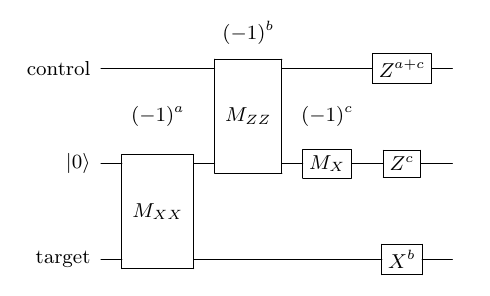
\includegraphics[scale=0.5]{img/cnotMeasureCircuit.png}\\
	\caption{A Quantum Circuit, where $|0\rangle$ is the +1
	eigenstate in $\sigma_z$-basis}
	\label{fig:circuit1}
	\end{center}
\end{figure}
\newpage

In the quantum circuit depicted in figure \ref{fig:circuit1} the input
state can be written as $|\psi_{control}\rangle \otimes |0\rangle 
\otimes |\psi_{target}\rangle$ and the measurement in the first 
timestep can be expressed as $\mathbb{I}\otimes X \otimes X$.\\
To simplify calculation we can write $|\psi_{target}\rangle$ as
$\alpha |+\rangle + \beta |-\rangle$, where $|+\rangle,|-\rangle$ are
the +1 and -1 Eigenstates of the $\sigma_x$-matrix. \\
The input state is thus: 
$|\psi_{control}\rangle \otimes |0\rangle 
\otimes( \alpha |+\rangle + \beta |-\rangle)$.\\
Upon the first measurement, if the measurement result on ancilla $|0\rangle$
is +1, the state becomes:
\begin{equation}
	|\phi^{+}_{t=1}\rangle = |\psi_{control}\rangle \otimes |+\rangle \otimes \alpha |+\rangle
\end{equation}
In this case, a = 0.
If the measurement result is -1, the state becomes:
\begin{equation}
	|\phi^{-}_{t=1}\rangle = |\psi_{control}\rangle \otimes |-\rangle \otimes \beta|-\rangle
\end{equation}
In this case, a = 1.\\
We now write $|\psi_{control}\rangle$ as $\gamma |0\rangle + \delta |1\rangle$
and $|\pm\rangle$ as $\frac{|0\rangle\pm|1\rangle}{\sqrt{2}}$.\\
Upon the second measurement then, if the measurement result on 
the control qubit is +1, and the first ancilla measurement was also +1, the state becomes:\\
\begin{equation}
	|\phi^{++}_{t=2}\rangle = \gamma |0\rangle \otimes |0\rangle \otimes \alpha |+\rangle
\end{equation}
Similarly:
\begin{equation}
	|\phi^{+-}_{t=2}\rangle = -\delta |1\rangle \otimes -|1\rangle \otimes \alpha |+\rangle
\end{equation}
\begin{equation}
	|\phi^{-+}_{t=2}\rangle = \gamma|0\rangle \otimes |0\rangle \otimes \beta|-\rangle
\end{equation}
\begin{equation}
	|\phi^{--}_{t=2}\rangle = -\delta|1\rangle \otimes |1\rangle \otimes \beta|-\rangle
\end{equation}
\\
In X basis, the state of the ancilla will be:\\
\begin{align}
	|\psi_A^{++}\rangle = \frac{|+\rangle+|-\rangle}{\sqrt{2}},
	|\psi_A^{+-}\rangle = \frac{|-\rangle-|+\rangle}{\sqrt{2}}\\
	|\psi_A^{-+}\rangle = \frac{|+\rangle+|-\rangle}{\sqrt{2}},
	|\psi_A^{--}\rangle = \frac{|+\rangle-|-\rangle}{\sqrt{2}}
\end{align}
Therefore, measuring X on the ancilla at t=3 will yield -1 or +1 both with probability
$\frac{1}{2}$ in the ++ and the -+ case, always -1 in the +- case and always +1 in the -- case.
\\
So then the target qubit will be resolved in the following way:
\begin{enumerate}
	\item $Z^{1+1} |\phi^{--}_{t=4}\rangle = -\delta|1\rangle \neq |\phi_{t=0}\rangle ???$
\end{enumerate}


\newpage
Meanwhile, in the Heisenberg picture we focus on the time-evolution of Operators:
\begin{equation}
	H = H(t)
\end{equation}
By specifically looking at the time evolution of those operators
to which the states in the system's input state space are 
eigenstates, we can figure out a systems output state space via:
\begin{equation}
	Circuit(\psi)=Circuit(H)\psi
\end{equation}

\newpage
\section{Conclusion}
In this thesis, we gave an overview of existing
quantum codes as well as some decoding schemes.
The determined thresholds of ca. 16\% for the surface/toric code were
within the literature expected range(ADD REFERENCE). 
Their thresholds were however not distinguishable, and
especially for the cylindric code in future works, it might be of interest to 
calculate these thresholds more precisely by using more significant computational
resources.
The pseudo-threshold for the Steane code was found to be around $10^{-5}$, which is
the same as in the literature\cite{steaneThreshold}. 
While the lifting decoder for the hexagonal toric lattice color code did not produce
thresholdable output, it did work as a proof-of-concept on smaller error vectors as in
\ref{fig: lifting}.
Future work could include adapting a better cycle-finder algorithm for the lifted 
subgraph.
\section{Appendix}
\subsection{Calculation 1}
\label{sec:calc1}

In the quantum circuit depicted in figure \ref{fig:circuit1} the input
state can be written as $|\psi_{control}\rangle \otimes |0\rangle 
\otimes |\psi_{target}\rangle$ and the measurement in the first 
timestep can be expressed as $\mathbb{I}\otimes X \otimes X$.\\
\\
The initial state $|\phi_{t=0}\rangle$ = $|\psi_{control}\rangle \otimes |\psi_{ancilla}\rangle \otimes
|\psi_{target}\rangle$\\
where\\
$|\psi_{control}\rangle = \alpha|0\rangle+\beta|1\rangle$
\\
$|\psi_{ancilla}\rangle = |0\rangle$
\\
$|\psi_{target}\rangle = \gamma|0\rangle+\delta|1\rangle$
\\
therefore:
\begin{equation}
|\phi_{t=0}\rangle = \alpha \left( \gamma |000\rangle + \delta |001\rangle\right)+
\beta \left( \gamma |100\rangle + \delta |101\rangle \right)
\end{equation}

If the first measurement result is +1, the state becomes:
\begin{align*}
	|\phi^{+}_{t=1}\rangle 
	&= \frac{1}{2}\left(\mathbb{I}\otimes\mathbb{I}\otimes\mathbb{I}+
	\mathbb{I}\otimes X \otimes X\right)|\phi_{t=0}\rangle\\
	&= \alpha \left( 
	\gamma \left( |000\rangle + |011\rangle \right) +
	\delta \left( |001\rangle + |010\rangle \right) \right) \\
	&+ \beta \left(
	\gamma \left( |100\rangle + |111\rangle \right) +
	\delta \left( |101\rangle + |110\rangle \right) \right)
\end{align*}
if the result is -1, it becomes:
\begin{align*}
	|\phi^{-}_{t=1}\rangle 
	&= \frac{1}{2}\left(\mathbb{I}\otimes\mathbb{I}\otimes\mathbb{I}-
	\mathbb{I}\otimes X \otimes X\right)|\phi_{t=0}\rangle\\
	&= \alpha \left( 
	\gamma \left( |000\rangle - |011\rangle \right) +
	\delta \left( |001\rangle - |010\rangle \right) \right) \\
	&+ \beta \left(
	\gamma \left( |100\rangle - |111\rangle \right) +
	\delta \left( |101\rangle - |110\rangle \right) \right)
\end{align*}

In the case of the +1 Measurement $\rightarrow$ a=0:
\begin{align*}
	|\phi^{++}_{t=2}\rangle 
	&= \frac{1}{2}\left(\mathbb{I}\otimes\mathbb{I}\otimes\mathbb{I}+
	Z\otimes Z \otimes \mathbb{I}\right)|\phi^{+}_{t=1}\rangle\\
	&= (|000\rangle\langle000| +|001\rangle\langle001| +
	|110\rangle\langle110| +|111\rangle\langle111|)|\phi^{+}_{t=1}\rangle\\
	&= \alpha \left( \gamma |000\rangle + \delta |001\rangle \right)
	+ \beta \left( \gamma |111\rangle + \delta |110\rangle\right) 
\end{align*}
\begin{align*}
	|\phi^{+-}_{t=2}\rangle 
	&= \frac{1}{2}\left(\mathbb{I}\otimes\mathbb{I}\otimes\mathbb{I}-
	Z \otimes Z \otimes \mathbb{I}\right)|\phi^{+}_{t=1}\rangle\\
	&= (|010\rangle\langle010| +|011\rangle\langle011| +
	|100\rangle\langle100| +|101\rangle\langle101|)|\phi^{+}_{t=1}\rangle\\
	&= \alpha \left( \gamma |011\rangle + \delta |010\rangle \right)
	+ \beta \left( \gamma |100\rangle + \delta |101\rangle \right) 
\end{align*}
In the case of the -1 Measurement $\rightarrow$ a=1:
\begin{align*}
	|\phi^{-+}_{t=2}\rangle 
	&= \frac{1}{2}\left(\mathbb{I}\otimes\mathbb{I}\otimes\mathbb{I}+
	Z\otimes Z \otimes \mathbb{I}\right)|\phi^{-}_{t=1}\rangle\\
	&= \alpha \left( \gamma |000\rangle + \delta |001\rangle \right)
	- \beta \left( \gamma |111\rangle + \delta |110\rangle\right) 
\end{align*}
\begin{align*}
	|\phi^{--}_{t=2}\rangle 
	&= \frac{1}{2}\left(\mathbb{I}\otimes\mathbb{I}\otimes\mathbb{I}-
	Z\otimes Z \otimes \mathbb{I}\right)|\phi^{-}_{t=1}\rangle\\
	&= - \alpha \left( \gamma |011\rangle + \delta |010\rangle \right)
	+ \beta \left( \gamma |100\rangle + \delta |101\rangle \right) 
\end{align*}
Now the applied measurement is 
$\mathbb{I} \otimes X \otimes \mathbb{I}$, which means:
\begin{align*}
	|\phi^{+++}_{t=3}\rangle 
	&= \frac{1}{2}\left(\mathbb{I}\otimes\mathbb{I}\otimes\mathbb{I}+
	\mathbb{I}\otimes X \otimes \mathbb{I}\right)|\phi^{++}_{t=2}\rangle\\
	&= \frac{1}{2}((|010\rangle + |000\rangle)\langle000|
	+ (|011\rangle + |001\rangle)\langle001|\\
	&+ (|000\rangle + |010\rangle)\langle010|
	+ (|001\rangle + |011\rangle)\langle011|\\
	&+ (|110\rangle + |100\rangle)\langle100|
	+ (|111\rangle + |101\rangle)\langle101|\\
	&+ (|100\rangle + |110\rangle)\langle110|
	+ (|101\rangle + |111\rangle)\langle111|)
	|\phi^{++}_{t=2}\rangle\\
	&= \frac{1}{2}(\alpha \left( 
	\gamma (|000\rangle + |010\rangle)+
	\delta (|011\rangle + |001\rangle) \right) \\
	&+ \beta \left( 
	\gamma (|101\rangle + |111\rangle)+
	\delta (|100\rangle + |110\rangle) \right))
\end{align*}
In this case, a,b and c would each be zero, therefore no further gate would be applied.\\
As intended, this state is equivalent to 
$CNOT_{|\psi_{Control}\rangle\rightarrow |\psi_{Target}\rangle} |\phi_{t=0}\rangle$.


\newpage
%\bibliographystyle{plain}
%\bibliography{references}
\end{document}

